\documentclass{article}[12pt]

%--------------Packages------------------------------
\usepackage[utf8]{inputenc} %Pour encoder du texte en français
\usepackage[francais]{babel} %Pour encoder du texte en français
\usepackage{graphicx} %pour inclure des images
\usepackage{version} % permet d'utiliser l'environnement comment
\graphicspath{{./figures/}} %repertoire images
\usepackage{listings} %si on veut afficher du code, le code doit se trouver dans un dossier "codes" 					  %lui même dans le même répertoire que ce fichier tex
\usepackage{color} %nécessaire pour changer les couleurs du highlighting du code
\usepackage{amsmath,amssymb}%pour des maths au cas où
\usepackage{array,multirow,makecell}%Pour manipuler les tableaux
\usepackage{url} %pour utiliser les liens hypertextes
\usepackage{hyperref} %pour utiliser les liens hypertextes
\usepackage{float}
\definecolor{dkgreen}{rgb}{0,0.6,0}
\definecolor{gray}{rgb}{0.5,0.5,0.5}
\definecolor{mauve}{rgb}{0.58,0,0.82}
\lstloadlanguages{SQL}

\lstset{frame=tb,
	inputpath={./codes/},
	language=SQL,
	aboveskip=3mm,
	belowskip=3mm,
	showstringspaces=false,
	columns=flexible,
	basicstyle={\small\ttfamily},
	numbers=none,
	numberstyle=\tiny\color{gray},
	keywordstyle=\color{blue},
	commentstyle=\color{dkgreen},
	stringstyle=\color{mauve},
	breaklines=true,
	breakatwhitespace=true,
	tabsize=3
}
%la macro a utilisé
\newcommand{\SQLcode}[2]{
	\begin{itemize}
		\item[]\lstinputlisting[caption=#2,label=#1]{#1.sql}
	\end{itemize}
}
\newlength{\length}
\setlength{\length}{3\baselineskip}

\newcommand{\Javacode}[2]{
	\begin{itemize}
    	\item[]\lstinputlisting[caption=#2,label=#1]{#1.java}
	\end{itemize}
}

% ---------- Document ------------ %
\begin{document}
	
	\begin{titlepage}

\newcommand{\HRule}{\rule{\linewidth}{0.5mm}} % Defines a new command for the horizontal lines, change thickness here

\center % Center everything on the page
 
%----------------------------------------------------------------------------------------
%	HEADING SECTIONS
%----------------------------------------------------------------------------------------

\textsc{\LARGE Institut Paul Lambin}\\[1.5cm] % Name of your university/college
\textsc{\Large BAC 2 Informatique de gestion}\\[0.5cm] % Major heading such as course name
\textsc{\large SQL}\\[0.5cm] % Minor heading such as course title

%----------------------------------------------------------------------------------------
%	TITLE SECTION
%----------------------------------------------------------------------------------------

\HRule \\[0.4cm]
{ \huge \bfseries Super-Heros-Y-Ena-La-Dedans }\\[0.4cm] % Title of your document
\HRule \\[1.5cm]
 
%----------------------------------------------------------------------------------------
%	AUTHOR SECTION
%----------------------------------------------------------------------------------------

\begin{minipage}{0.4\textwidth}
\begin{flushleft} \large
\emph{Auteurs:}\\
Christopher \textsc{Sacré} \\
Damien \textsc{Meur} % Your name
\end{flushleft}
\end{minipage}
~
\begin{minipage}{0.4\textwidth}
\begin{flushright} \large
\emph{Professeur:} \\
D. \textsc{Grolaux} % Supervisor's Name
\end{flushright}
\end{minipage}\\[4cm]

% If you don't want a supervisor, uncomment the two lines below and remove the section above
%\Large \emph{Author:}\\
%John \textsc{Smith}\\[3cm] % Your name

%----------------------------------------------------------------------------------------
%	DATE SECTION
%----------------------------------------------------------------------------------------

{\large \today}\\[3cm] % Date, change the \today to a set date if you want to be precise

%----------------------------------------------------------------------------------------
%	LOGO SECTION
%----------------------------------------------------------------------------------------

%\includegraphics{Logo}\\[1cm] % Include a department/university logo - this will require the graphicx package
 
%----------------------------------------------------------------------------------------

\vfill % Fill the rest of the page with whitespace

\end{titlepage}
	
	\tableofcontents%table des matières
	\newpage
	
	
	%différentes sections
	\section{Introduction}
	Pour l'unité d'enseignement de Gestion des données et plus précisément pour le cours de SQL, il nous a été demandé de réaliser une application en PostgreSQl et Java. Cette application comprend 2 acteurs principaux : les agents du SHYELD qui disposent d'un application Java pour :
	\begin{itemize}
		\item Disposer des informations des super-héros et d'ajouter ceux-ci en cas d'absence dans la base de données
		\item Ajouter des repérages de super-héros
		\item Ajouter des combats et les participations qui y sont liés
		\item Remarquer la mort d'un super-héros
	\end{itemize}
	; ainsi qu'une application centrale, elle aussi programmée en Java pour l'interface utilisateur, elle permet :
	\begin{itemize}
		\item Inscrire des agents
		\item Supprimer des agents
		\item Disposer d'informations sur la perte de visibilité de super-héros
		\item Remarquer la mort d'un super-héros
		\item Lister des zones de conflits
		\item Relever l'historique des repérages d'un agent
		\item Disposer de statistiques de gestions tels que : le classement de victoires/défaites des super-héros ou le classement du nombre de repérages effectués par les agents.
	\end{itemize}
	Nous expliquerons dans ce rapport certains de nos choix d'implémentations pour réaliser ce projet.
	\section{Remarques globales}
	\subsection{Diagramme de structures des données}
	\begin{figure}[H]
		\centering
		\fbox{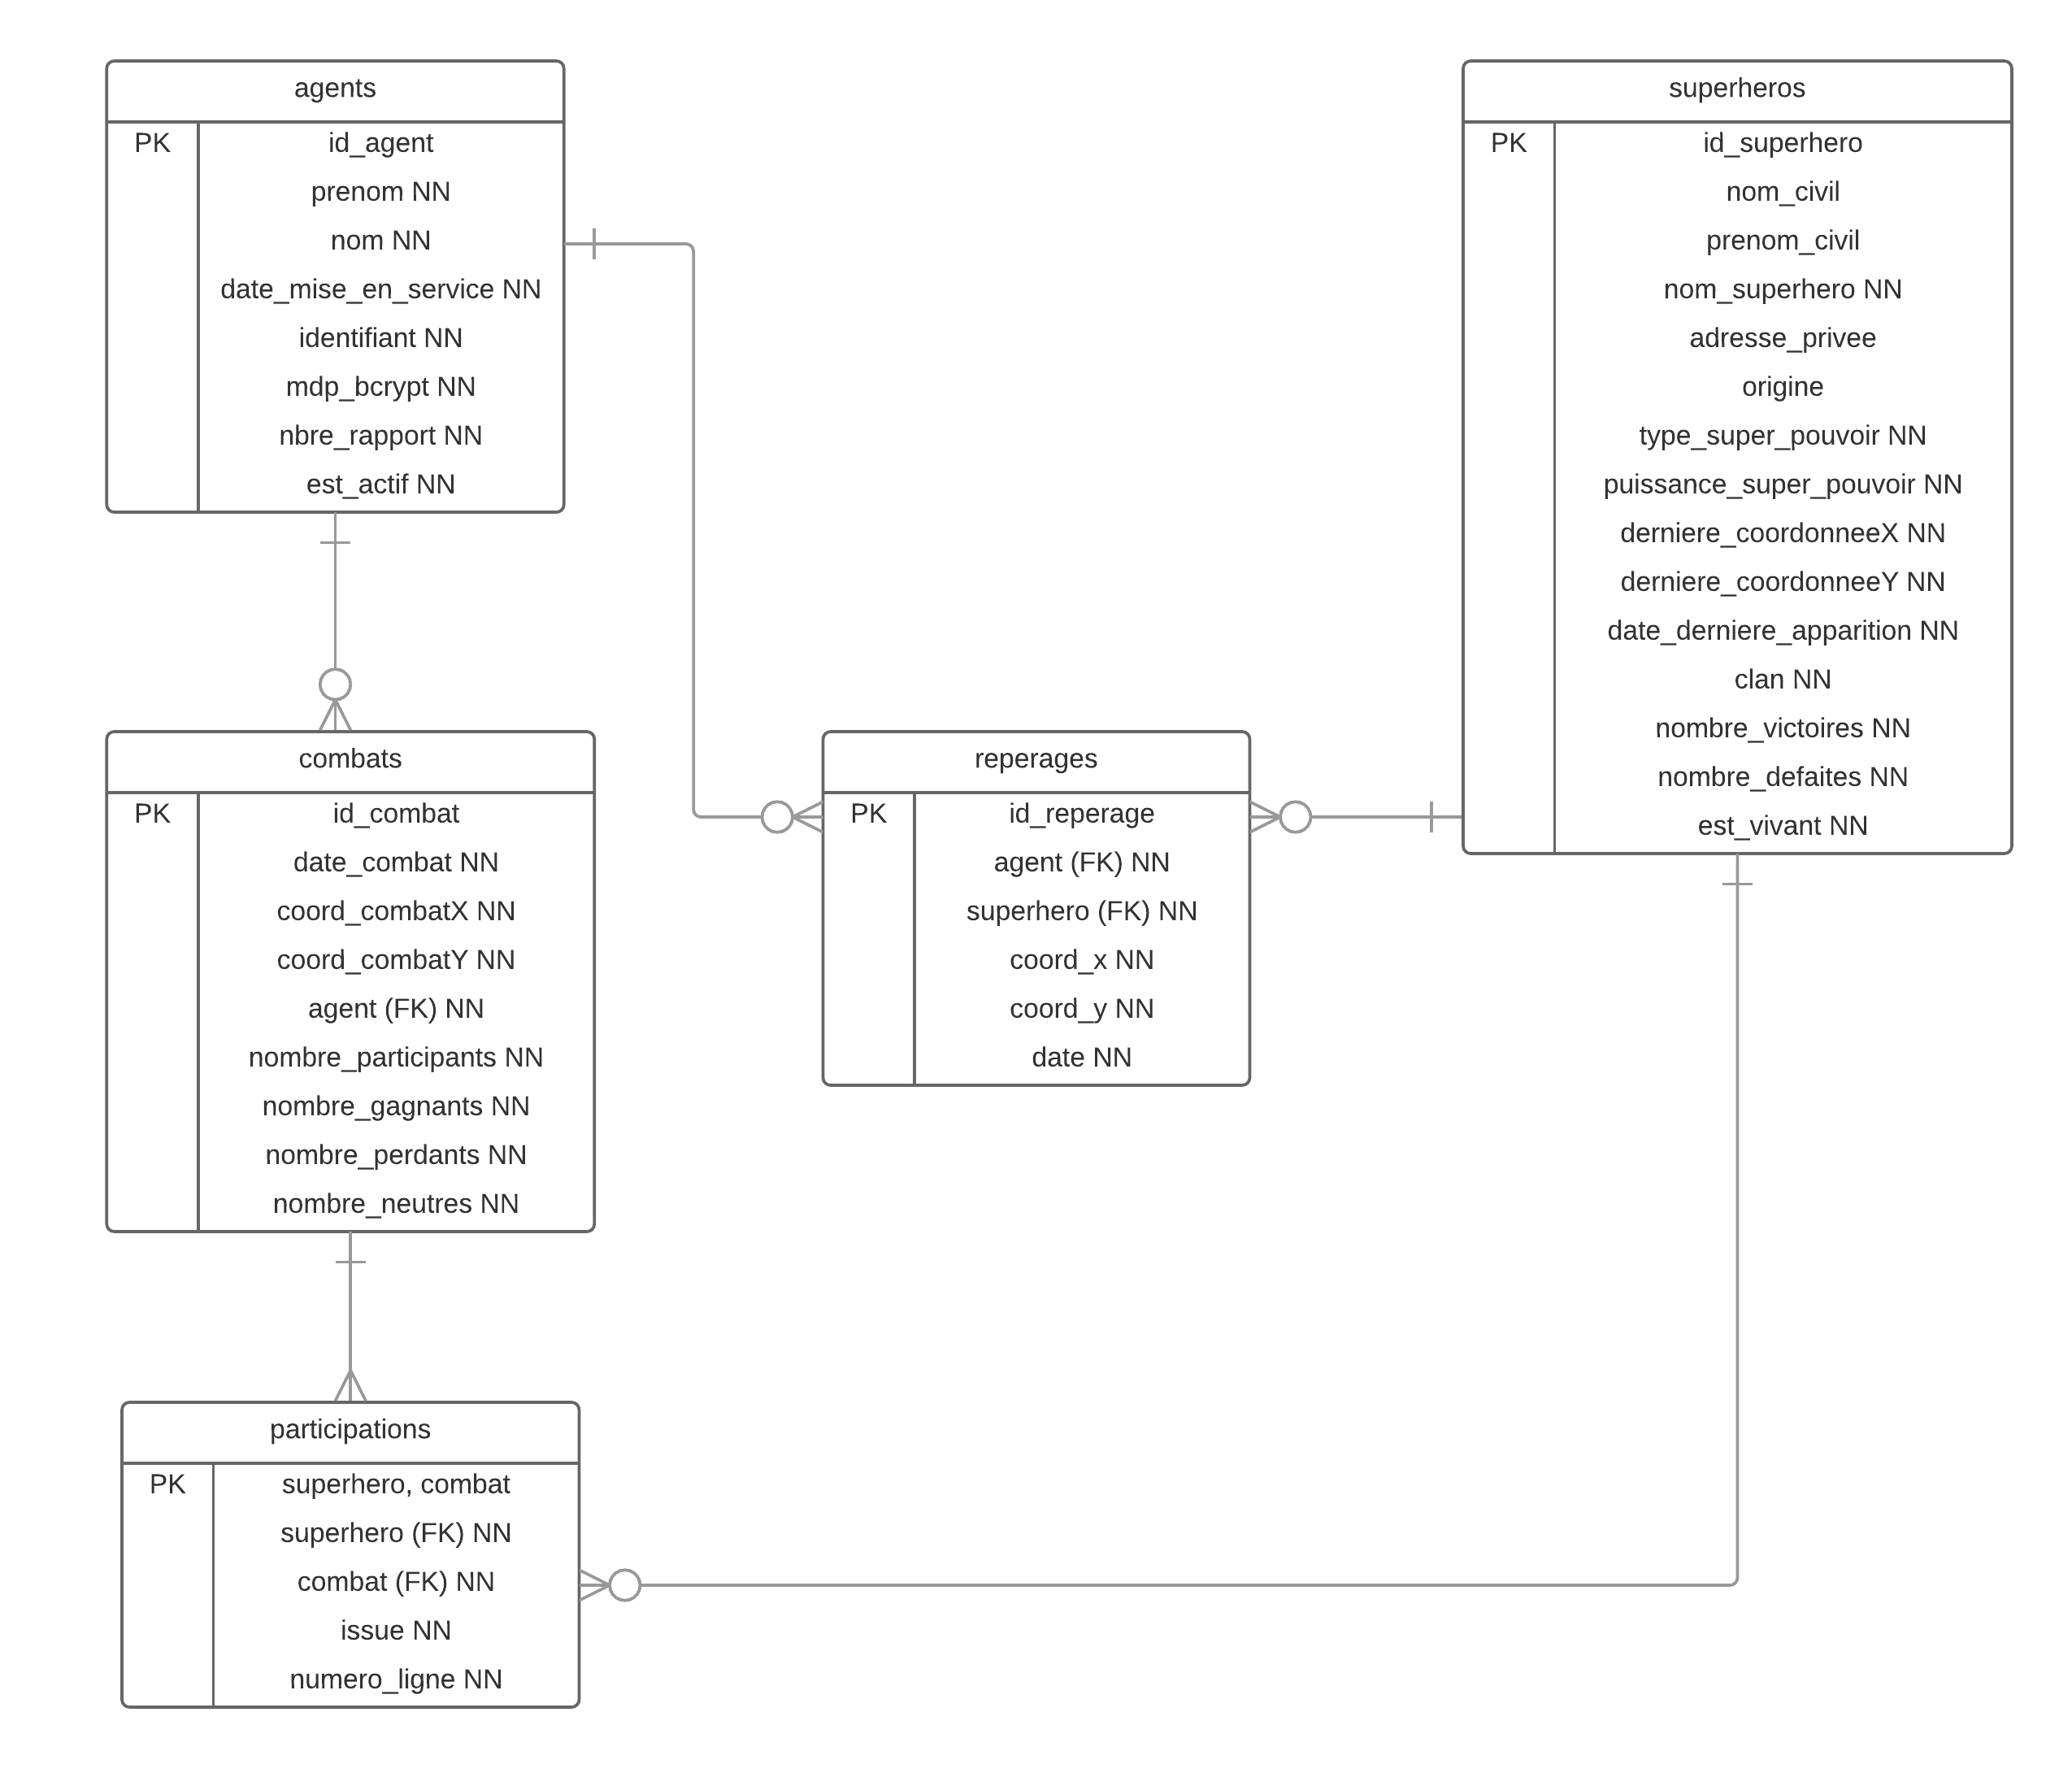
\includegraphics[width=\textwidth,height=12cm]{dsd.png}}
		\caption{Page d'accueil du bug}
	\end{figure}
    \newpage
	\subsection{Description du diagramme de structures des données}
	\label{dsd}
	Nous avons fait le choix de dénormaliser les champs suivants: 
	\begin{itemize}
		\item nbre\_rapport (table agents)
		\item nombre\_participants (tables combats)
		\item nombre\_gagnants (table combats)
		\item nombre\_perdants (tables combats)
		\item nombre\_neutres (table combats)
		\item nombre\_victoires (table superheros)
		\item nombre\_defaites (table superheros)
		\item date\_derniere\_apparition (table superheros)
		\item derniere\_coordonneeX (table superheros) 	
		\item derniere\_coordonneeY (table superheros) 	
	\end{itemize}
	\paragraph{Encryption}
	Le mot de passe des agents (indispensable pour leur permettre de se connecter à l'application) est encrypté grâce à une clé \textit{BCRYPT}.
	\paragraph{Suppression des données}
	Pour éviter d'avoir des participations qui ne soient liées à aucun super-héros et à aucun agent, nous avons utilisé un système de drapeau (\textit{est\_vivant} \& \textit{est\_actif}).
	
	\subsection{Vérification des données primaires}
	Lors de la création des tables, nous avons veillé à effectuer quelques vérifications essentielles (d'autres plus avancées à base de \textit{TRIGGER} seront détaillées dans les sections \ref{shyield} et\ref{agent} ).
	Pour la table superheros : 
	\begin{itemize}
		\item Aucune chaîne de caractère ne doit être vide
		\item La puissance d'un super pouvoir doit être comprise entre 1 et 10.
		\item Les coordonnées doivent être comprises entre 1 et 100.
		\item Le nombre de victoires et défaites doivent être supérieur ou égal à 0.
		\item La date de dernière apparition doit être inférieure ou égale à la date actuelle du serveur.
        \item Un clan ne peut être que 'M' (Marvelle) ou 'D' (Décé).
	\end{itemize}
	Pour la table agents :
	\begin{itemize}
		\item Les chaînes de caractères ne peuvent pas être vides.
		\item Les date de mise en service doit être inférieure ou égale à la date du serveur.
		\item Le nombre de rapports doit être supérieur ou égal à 0.
	\end{itemize}
	Pour la table combats:
	\begin{itemize}
		\item La date du combat doit être inférieure  ou égale à la date du serveur.
		\item Les coordonnées doivent être comprises entre 0 et 100.
		\item Le nombre de participants doit être supérieur ou égal au nombre de perdants et de gagnants ( il est possible d'avoir des participations neutres à un combat) et supérieur ou égal à 0.
		\item Le nombre de gagnants, de perdants et de participations neutres pour un combat doivent être supérieur ou égal à 0.
	\end{itemize}
	Pour la table participations :
	\begin{itemize}
		\item L'issue d'un combat vaut 'N' (neutre) par défaut. L'issue d'un combat dépend doit valoir 'N', 'P' (perdant) ou 'G' (gagnant). Un type a été créé à cet effet.
		\item Le numéro de ligne est plutôt ici à titre informatif et peut être utilisé afin de trier l'affichage d'un combat.
	\end{itemize}
	Pour la table repérages
	\begin{itemize}
		\item Les coordonnées doivent être comprises entre 0 et 100.
		\item La date doit être inférieur (ou égale) à la date du serveur.
	\end{itemize}
	\subsection{Affichage des données au sein de la console JAVA}
	Actuellement nous avons d'utiliser la classe \href{https://github.com/htorun/dbtableprinter}{DBTablePrinter} afin d'afficher les résultats de la plupart de nos requêtes au sein de console. Cela permet notamment d'avoir un affichage clair du résultat. D'autres requêtes ne renvoyant qu'un tuple d'une colonne pour résultat sont quant à elle affichées directement dans la console sans passer par la classe DBTablePrinter (résultat des insertions dans la base de données, ...).
    \subsection{Gestion des Transactions lors de l'ajout d'un combat}
    L'ajout d'un combat se fait au sein d'une transaction reprenant le combat en tant que tel ainsi que les participations qui y sont rattachées. Cela permet notamment d'effectuer plusieurs tests afin d'empêcher l'insertion d'un combat invalide.
   	\Javacode{transaction}{Utilisation de transaction au sein de notre application}
    \subsection{Utilisation de VIEWS au sein de notre code}
    Pour certaines opérations ne nécessitant aucune donnée, nous avons préféré utiliser des vues plutôt qu'une procédure à proprement parler, c'est notamment le cas pour : 
    \SQLcode{perte_visibilite}{Obtenir les informations sur tous les héros n'ayant pas été aperçu depuis plus de dix jours}
    \SQLcode{zone_conflit}{Lister les zones potentielles de conflit}
    \SQLcode{classement_victoires}{Obtenir un classement des héros en fonction de leurs victoires}
    \SQLcode{classement_defaites}{Obtenir un classement des héros en fonction de leurs défaites}
    
   \SQLcode{classement_reperages}{Obtenir un classement des héros en fonction de leurs repérages}
   
\SQLcode{affichage_agents}{Afficher le contenu de la table shyeld.agents}

\SQLcode{affichage_combats}{Afficher le contenu de la table shyeld.combats}

\SQLcode{affichage_reperages}{Afficher le contenu de la table shyeld.reperages}
    
	\section{Remarques application SHYELD}
	\label{shyield}
	\subsection{SQL}
		
	\subsubsection{Triggers nécessaires à la dénormalisation}
	
Etant donné que certains champs sont dénormalisés (voir section \ref{dsd}), nous avons utilisés des triggers pour les tenir à jour.

 La vérification des données d'un combat se fait par exemple via la fonction \textit{shyeld.verificationAuthenticiteCombat()}. Le déclenchement de ce trigger nous a posé soucis car les combats et les participations sont ajoutés au sein d'une transaction. Nous avons dès lors ajouté l'option "DEFERRABLE INITIALLY DEFERRED" dans la déclaration de notre trigger. Il est à noter que le nombre de rapports de l'agent est incrémenté directement depuis la fonction de création de combat.
 	\SQLcode{triggerCombat}{Trigger de vérification d'un combat}
 	
 Lors de la création d'un combat, chaque participation entraîne la création automatique d'un repérage. Si le combat n'est pas valide (il n'y a pas au moins un héros de chaque clan), la transaction sera annulée (ROLLBACK). En cas de combat invalide (inexistance d'au moins deux participations de deux héros de clans adverses), les repérages liés aux transactions sont tout de même effectués.
 	\SQLcode{triggerReperage}{Trigger de création automatique de repérage en cas d'insertion d'une participation}
 
	
	\subsubsection{Droits d'accès aux données}
	Etant donné que l'application SHYELD est l'application centrale, elle sera exécutée grâce à l'utilisateur POSTGRESQL possédant la base de donnée, aucune restriction d'accès n'est effectuée pour cette partie de l'application.
	\subsection{Java}
	
	
	\section{Remarques application Agent}
	\label{agent}
	\subsubsection{SQL}

	\subsubsection{Connexion Agent}
	Etant donné que les mots de passes sont salés, nous faisons la vérfication de ceux-ci en Java. La fonction s shyeld.check\_connexion(varchar(255)) renvoie le mot de passe haché en BCRYPT pour faire la vérification au sein de l'applicaiton java (elle renvoie NULL en cas où 'identifiant ne correspond à aucun utilisateur.
	\subsubsection{Droits d'accès aux données}
	L'agent n'est pas considéré comme un utilisateur administrateur, nous avons donc minimisé ces droits d'accès à la base de données au minium. A noter que l'utilisateur administrateur est représenté ici par \textit{dmeur15} et l'utisateur agent par \textit{csacre15}.
	\SQLcode{grant}{Droits d'accès à la base de données pour un agent}
	\subsection{Java}
	
\end{document}
